\documentclass[9pt]{beamer}
\beamertemplatenavigationsymbolsempty
\usetheme{Berlin}

\usepackage{etex, tikz, array, graphics, xspace, relsize, multirow}
\usepackage{ulem}

\input binhex

% For code inclusion
\usepackage{listings}
\lstset{ breaklines=true}
\lstset{escapeinside={<@}{@>}}
\usepackage{algorithm2e}
\usepackage{algorithmic}

% Commands
\newcommand\A{\mathcal{A}}
\newcommand\cc{\mathcal{C}}
\newcommand\codim{\mathrm{codim}}
\newcommand\CP{\mathbb{CP}}
\newcommand\C{\mathbb{C}}
\newcommand\D{\mathrm{D}}
\newcommand\hto{\hookrightarrow}
\newcommand\I{^{-1}}
\newcommand\oo{\mathcal{O}}
\renewcommand\phi{\varphi}
\newcommand\Pj{\mathbb{P}}
\newcommand\pow{\mathcal{P}}
\newcommand\RP{\mathbb{RP}}
\newcommand\rstr[2]{{\left.#1\right|_{#2}}}
\newcommand\R{\mathbb{R}}
\newcommand\V{\mathcal{V}}
\newcommand\H{\mathcal{H}}
\newcommand\set[1]{\{#1\}}
\newcommand\toi{\xrightarrow{\sim}} % category
\newcommand\Z{\mathbb{Z}}


% For drawing
%% Tikz drawing
\usepackage{tikz}
\usetikzlibrary{arrows}
\usetikzlibrary{arrows.meta}
\usepackage{pgfplots}
\usepackage{tikz-3dplot}
\usepackage{tcolorbox}
\usetikzlibrary{matrix,fit,positioning,shapes.geometric,patterns,backgrounds}
\usetikzlibrary{decorations.pathreplacing}
\usetikzlibrary{decorations.markings}
\usetikzlibrary{arrows,calc}
\tikzstyle{bigbox} = [draw=blue!50, thick, rounded corners, rectangle]
\tikzset{
>=stealth'
}
\tikzset{->-/.style={decoration={
  markings,
  mark=at position #1 with {\arrow{>}}},postaction={decorate}}}

%% Software names
\newcommand\topcom{\texttt{TOPCOM}\xspace}
\newcommand\mptopcom{\texttt{MPTOPCOM}\xspace}
\newcommand\mptopcomone{\texttt{MPTOPCOM-1}\xspace}
\newcommand\mts{\texttt{mts}\xspace}
\newcommand\mplrs{\texttt{mplrs}\xspace}
\newcommand\soplex{\texttt{soplex}\xspace}
\newcommand\openmpi{\texttt{OpenMPI}\xspace}
\newcommand\mpi{\texttt{MPI}\xspace}
\newcommand\gfan{\texttt{Gfan}\xspace}
\newcommand\cddlib{\texttt{cddlib}\xspace}
\newcommand\polydb{\texttt{PolyDB}\xspace}
\newcommand\oscar{\texttt{OSCAR}\xspace}

\usepackage{xcolor}
\definecolor{green}{rgb}{0.1,0.59,0.1}
\definecolor{yellow}{rgb}{0.8,0.67,0}
\definecolor{red}{rgb}{0.89,0.1,0.1}
\definecolor{blue}{rgb}{0.1,0.1,0.89}

\usenavigationsymbolstemplate{}

\usepackage{booktabs}
% For software citations
\newcommand{\polymake}{\texttt{po\-ly\-ma\-ke}\xspace}
\newcommand{\polymakejl}{\texttt{Po\-ly\-ma\-ke.jl}\xspace}
\newcommand{\singular}{\texttt{Sin\-gu\-lar}\xspace}
\newcommand\CPP{C\nolinebreak\hspace{-.05em}\raisebox{.4ex}{\relsize{-3}{\textbf{+}}}\nolinebreak\hspace{-.10em}\raisebox{.4ex}{\relsize{-3}{\textbf{+}}}\xspace}

\usepackage{amsmath}
% Newcommands specifically for this article
\newcommand{\eval}{v}               % evaluation function giving switch table
\newcommand{\graph}{\Gamma}         % reverse search graph
\newcommand{\group}{G}              % group acting on point config
\newcommand{\groupElem}{g}          % element of group
\newcommand{\jbound}{\psi}          % bound on the number of elements of set J
\newcommand{\switchTableSize}{\mu}  % index of last non-trivial row in switch table

\newcommand{\pc}{\mathcal P\mathcal C}
\newcommand{\ZZ}{\mathbb Z}
\renewcommand{\AA}{\mathcal A}
\newcommand{\QQ}{\mathbb Q}
\newcommand{\OO}{\mathcal O}
\newcommand{\CC}{\mathbb C}
\newcommand{\PP}{\mathbb P}
\newcommand{\RR}{\mathbb R}
\newcommand{\scalp}[1]{\langle #1 \rangle}
\newcommand{\wt}{\omega}
\newcommand{\cT}{\mathcal T}
\renewcommand{\O}{\mathcal O}
\newcommand{\adm}{\mathcal A(\D, M)}
\newcommand{\blue}[1]{{\usebeamercolor[fg]{palette primary}#1}}

\DeclareMathOperator{\CaDiv}{CaDiv}
\DeclareMathOperator{\conv}{conv}
\DeclareMathOperator{\below}{defect}
\DeclareMathOperator{\vertex}{vertex}
\DeclareMathOperator{\Cox}{Cox}
\DeclareMathOperator{\cl}{cl}
\DeclareMathOperator{\cone}{cone}
\DeclareMathOperator{\Ext}{Ext}
\DeclareMathOperator{\Tor}{Tor}
\DeclareMathOperator{\lcm}{lcm}
\DeclareMathOperator{\Quot}{Quot}
\DeclareMathOperator{\Spec}{Spec}
\DeclareMathOperator{\Sets}{Sets}
\DeclareMathOperator{\relint}{relint}
\DeclareMathOperator{\rk}{rk}
\DeclareMathOperator{\smallestFace}{smallestFace}
\DeclareMathOperator{\Pic}{Pic}
\DeclareMathOperator{\Hom}{Hom}
\DeclareMathOperator{\vol}{vol}
\DeclareMathOperator{\TV}{TV}
\DeclareMathOperator{\tail}{tail}
\DeclareMathOperator{\rep}{rep}
\DeclareMathOperator{\vspan}{span}
\DeclareMathOperator{\canonical}{can}
\DeclareMathOperator{\gkz}{gkz}

\newcommand{\pmsmall}{
\includegraphics[scale=0.03]{pmlogo.png}}
\newcommand{\pmlogo}{
\includegraphics[scale=0.09]{pmlogo.png}}
\newcommand{\pmbluesmall}{\includegraphics[scale=0.03]{pmbluelogo.png}}
\newcommand{\Disjoint}{\mathop{\coprod}}
\newcommand{\Discriminant}{\mathcal{D}}

\theoremstyle{definition}
\newtheorem{remark}{Remark}

\newtheorem{prop}{Proposition}
\newtheorem{defn}{Definition}

\author{Antony Della Vecchia}
\title{Computing Convex Hulls}
%\newtheorem*{example}{Example}
\institute[]{
Technische Universit\"at Berlin
}
\date{
2022-10-12
}


\newcommand{\surj}{\twoheadrightarrow}
\newcommand{\oursetting}[1]{\textcolor{blue}{#1}}
\usepackage{listings}
\begin{document}
\maketitle
%%%%%%%%%%%%%%%%%%%%%%%%%%%%%%%%%%%%%%%%%%%%%%%%%%%%%%%%%%%%%%%%%%%%%%%%%%%%%%%
%%%%%%%%%%%%%%%%%%%%%%%%%%%%%%%%%%%%%%%%%%%%%%%%%%%%%%%%%%%%%%%%%%%%%%%%%%%%%%%
%%%%%%%%%%%%%%%%%%%%%%%%%%%%%%%%%%%%%%%%%%%%%%%%%%%%%%%%%%%%%%%%%%%%%%%%%%%%%%%
\begin{frame}[fragile]{Overview}
  \begin{tcolorbox}
    \tableofcontents
  \end{tcolorbox}
\end{frame}
%%%%%%%%%%%%%%%%%%%%%%%%%%%%%%%%%%%%%%%%%%%%%%%%%%%%%%%%%%%%%%%%%%%%%%%%%%%%%%%
%%%%%%%%%%%%%%%%%%%%%%%%%%%%%%%%%%%%%%%%%%%%%%%%%%%%%%%%%%%%%%%%%%%%%%%%%%%%%%%
%%%%%%%%%%%%%%%%%%%%%%%%%%%%%%%%%%%%%%%%%%%%%%%%%%%%%%%%%%%%%%%%%%%%%%%%%%%%%%%

%%%%%%%%%%%%%%%%%%%%%%%%%%%%%%%%%%%%%%%%%%%%%%%%%%%%%%%%%%%%%%%%%%%%%%%%%%%%%%%
\section{Preliminaries}
%%%%%%%%%%%%%%%%%%%%%%%%%%%%%%%%%%%%%%%%%%%%%%%%%%%%%%%%%%%%%%%%%%%%%%%%%%%%%%%

\begin{frame}[fragile]{Hulls}
  \begin{defn}
    Let $A \subset \mathbb{K}^n$, an \emph{affine combination} of points in $A$
    is a linear combination $\sum_{i=1}^m \lambda_m a_m$ where $\lambda_m \in
    \mathbb{K}$ and $a \in A$ such that $\sum_{i=1}^m \lambda_m = 1$. The
    \emph{affine hull} is the set of all such combinations.
  \end{defn}

  \begin{defn}
    Let $A \subset \mathbb{R}^n$, a \emph{convex combination} of points in $A$
    is an affine combination $\sum_{i=1}^m \lambda_m a_m$ where $\lambda_m \geq
    0$. The  \emph{convex hull} is the set of all such combinations.
  \end{defn}

  \begin{defn}
    Let $A \subset \mathbb{R}^n$, a \emph{postive combination} of points in $A$
    is a linear combination $\sum_{i=1}^m \lambda_m a_m$ where $\lambda_m \geq
    0$. The  \emph{positive hull} is the set of all such combinations.
  \end{defn}
\end{frame}
%%%%%%%%%%%%%%%%%%%%%%%%%%%%%%%%%%%%%%%%%%%%%%%%%%%%%%%%%%%%%%%%%%%%%%%%%%%%%%%
%%%%%%%%%%%%%%%%%%%%%%%%%%%%%%%%%%%%%%%%%%%%%%%%%%%%%%%%%%%%%%%%%%%%%%%%%%%%%%%
%%%%%%%%%%%%%%%%%%%%%%%%%%%%%%%%%%%%%%%%%%%%%%%%%%%%%%%%%%%%%%%%%%%%%%%%%%%%%%%

\begin{frame}[fragile]{}
  \begin{defn}
    \begin{itemize}
    \item Let $(x_0, \dots x_n) \in \mathbb{K}^{n+1} \setminus 0$, and let $x := \text{lin}{(x_0, \dots, x_n)}$,
      for any element of $x \setminus 0$ we call $(x_0: \dots :x_n)$ \emph{homegeneous coordinates} for $x$,
      with $(y_0: \dots y_n) \sim (x_0: \dots x_n)$ if $\lambda (x_0, \dots, x_n) = (y_0, \dots, y_n)$ with $\lambda \neq 0$, we call equivalence classes with a the first coefficient $0$ \emph{ideal points}.
    \item Given a linear transformation $A \in \text{GL}(\mathbb{K}, n+1)$ we call the induced transformation on homogeneous coordinates a \emph{projective transformation}.
    \item We call a transformation \emph{affine} if it sends ideal points to ideal points.
    \end{itemize}
  \end{defn}
  \begin{center}
    \includegraphics[width=.70\textwidth, height=0.3\textheight]{images/projectivize}
  \end{center}

\end{frame}
%%%%%%%%%%%%%%%%%%%%%%%%%%%%%%%%%%%%%%%%%%%%%%%%%%%%%%%%%%%%%%%%%%%%%%%%%%%%%%%
%%%%%%%%%%%%%%%%%%%%%%%%%%%%%%%%%%%%%%%%%%%%%%%%%%%%%%%%%%%%%%%%%%%%%%%%%%%%%%%
%%%%%%%%%%%%%%%%%%%%%%%%%%%%%%%%%%%%%%%%%%%%%%%%%%%%%%%%%%%%%%%%%%%%%%%%%%%%%%%

\begin{frame}[fragile]{Polytopes}
  \begin{defn}
    A set $P \subset \mathbb{R}^n$ is a \emph{polytope} if it can be described
    as the convex hull of finitely many points. The dimension of $P$ is
    defined to be the dimension of it's affine hull. A \emph{$k$-polytope} is a
    k dimensional polytope. A \emph{$k$-simplex} is the convex hull of $k + 1$
    affine independant points.
  \end{defn}

  \begin{figure}
    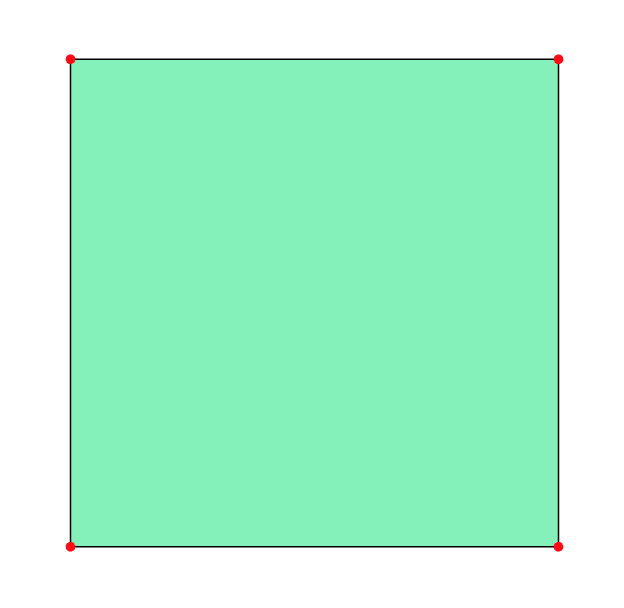
\includegraphics[width=.30\textwidth, height=0.4\textheight]{images/square}
    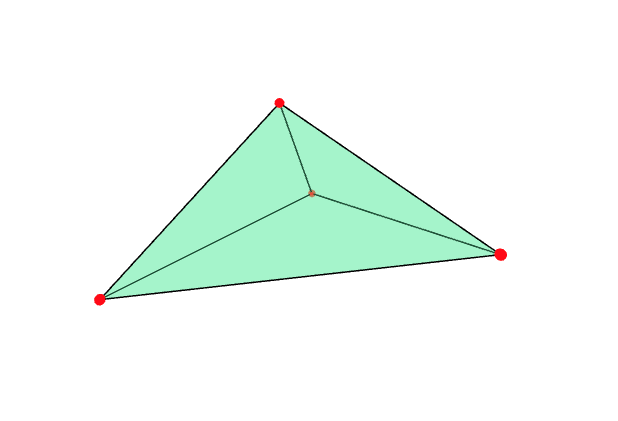
\includegraphics[width=.30\textwidth, height=0.4\textheight]{images/simplex}
  \end{figure}

\end{frame}
%%%%%%%%%%%%%%%%%%%%%%%%%%%%%%%%%%%%%%%%%%%%%%%%%%%%%%%%%%%%%%%%%%%%%%%%%%%%%%%
%%%%%%%%%%%%%%%%%%%%%%%%%%%%%%%%%%%%%%%%%%%%%%%%%%%%%%%%%%%%%%%%%%%%%%%%%%%%%%%
%%%%%%%%%%%%%%%%%%%%%%%%%%%%%%%%%%%%%%%%%%%%%%%%%%%%%%%%%%%%%%%%%%%%%%%%%%%%%%%


\begin{frame}[fragile]{Faces}
  \begin{defn}
    Given an n-polytope $P \subset \mathbb{R}^n$, the intersection $P \cap H$
    with a supporting hyperplane $H$ is called a \emph{proper face}. A face of
    dimension $k$ is called a $k$ face, a 0-face is a vertex, 1-face an edge,
    $n-2$-face a ridge and an $n-1$-face a facet.
  \end{defn}
  \begin{remark}
    Proper faces are also polytopes with respect to their affine hull.
  \end{remark}
  \begin{theorem}
    The boundary of a full dimesional polytope is the union of all it's
    proper faces.
  \end{theorem}

\end{frame}
%%%%%%%%%%%%%%%%%%%%%%%%%%%%%%%%%%%%%%%%%%%%%%%%%%%%%%%%%%%%%%%%%%%%%%%%%%%%%%%
%%%%%%%%%%%%%%%%%%%%%%%%%%%%%%%%%%%%%%%%%%%%%%%%%%%%%%%%%%%%%%%%%%%%%%%%%%%%%%%
%%%%%%%%%%%%%%%%%%%%%%%%%%%%%%%%%%%%%%%%%%%%%%%%%%%%%%%%%%%%%%%%%%%%%%%%%%%%%%%

\begin{frame}[fragile]{Half-spaces}
  \begin{defn}
    Given an affine hyperplane $H \subset \mathbb{R}^n$ given in homogeneous
    coordinates as $[a_0 : \dots : a_n]$, define the \emph{positive halfspace}
    $H^+$ as $\{x \in \mathbb{R}^n \mid a_0 + a_1x_1 + \dots + a_nx_n \geq 0 \}$.
  \end{defn}

  \begin{remark}
    For each facet $f$ of a polytope $P$, there exists a positive halfspace $H^+$
    such that $f = P \cap H$ and $ P \subset H^+$
  \end{remark}

  \begin{center}
    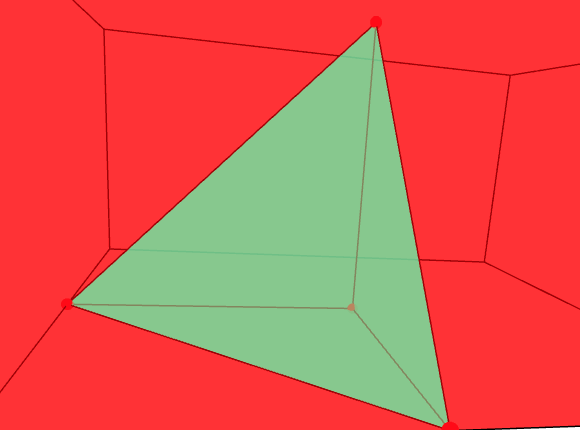
\includegraphics[width=.30\textwidth, height=0.4\textheight]{images/half-space}
  \end{center}
\end{frame}
%%%%%%%%%%%%%%%%%%%%%%%%%%%%%%%%%%%%%%%%%%%%%%%%%%%%%%%%%%%%%%%%%%%%%%%%%%%%%%%
%%%%%%%%%%%%%%%%%%%%%%%%%%%%%%%%%%%%%%%%%%%%%%%%%%%%%%%%%%%%%%%%%%%%%%%%%%%%%%%
%%%%%%%%%%%%%%%%%%%%%%%%%%%%%%%%%%%%%%%%%%%%%%%%%%%%%%%%%%%%%%%%%%%%%%%%%%%%%%%

\begin{frame}[fragile]{Polytope Descriptions}
  \begin{theorem}
    Let $H_i$ be the supporting hyperplanes for the facets of a polytope $P$.
    then $P = \cap_i^m H_i^+$
  \end{theorem}
  \begin{theorem}
    Every polytope is the convex hull of it's vertices
  \end{theorem}
  \begin{remark}
    We call $P =  \text{conv}(v_1, \dots, v_m)$ a $V$-description, and
    we call $P =  \cap_{i=1}^kH_i^+$ an $\mathcal{H}$-description. An algorithm
    that finds a $V$-description from an $\mathcal{H}$-description is referred to as a convex
    hull computation. We call the pair ${V, \mathcal{H} }$ a double description of $P$.
  \end{remark}
\end{frame}
%%%%%%%%%%%%%%%%%%%%%%%%%%%%%%%%%%%%%%%%%%%%%%%%%%%%%%%%%%%%%%%%%%%%%%%%%%%%%%%
%%%%%%%%%%%%%%%%%%%%%%%%%%%%%%%%%%%%%%%%%%%%%%%%%%%%%%%%%%%%%%%%%%%%%%%%%%%%%%%
%%%%%%%%%%%%%%%%%%%%%%%%%%%%%%%%%%%%%%%%%%%%%%%%%%%%%%%%%%%%%%%%%%%%%%%%%%%%%%%


\begin{frame}[fragile]{Polarity and Duality}
  \begin{defn}
    Given a set $X \subset \mathbb{R}^n$ define the polar set as
    $X^o = \{y \in \mathbb{R}^n \mid x_1y_1 + \dots x_ny_n \leq 1\}$
  \end{defn}
  \begin{theorem}
    If $P \subset \mathbb{R}^n$ is an $n$-polytope with $0 \in \text{int}P$ then
    $P^o$ is also an $n$-polytope, and for $V$ the vertex set of $P$ we have
    \begin{center}
      $P^o = \bigcap_{v \in V} \set{y \in \R^n \mid \langle v, y \rangle \leq 1} = \bigcap_{v \in V} [1: -v_0: \dots : -v_n]^+$
    \end{center}
  \end{theorem}
  \begin{center}
    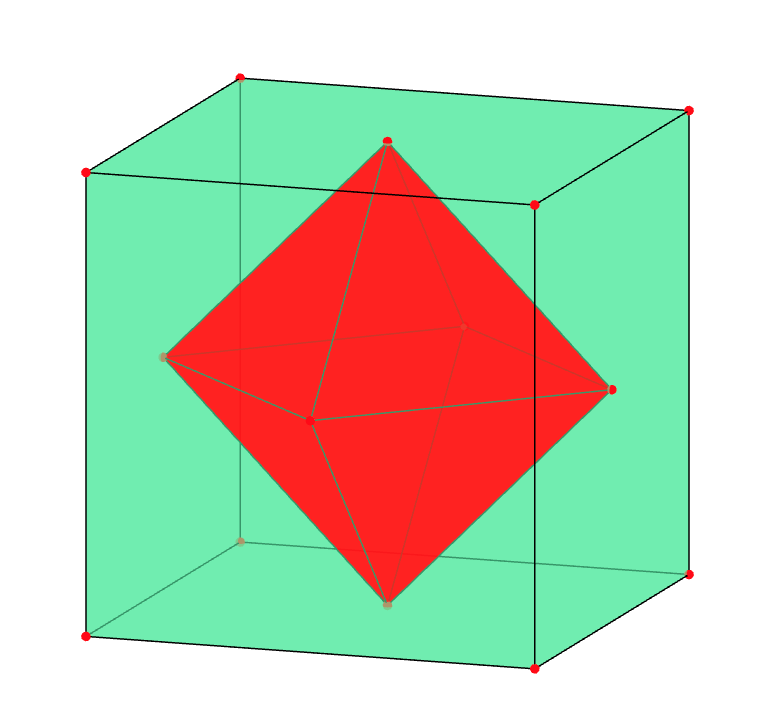
\includegraphics[width=.30\textwidth, height=0.4\textheight]{images/polar}
  \end{center}
\end{frame}
%%%%%%%%%%%%%%%%%%%%%%%%%%%%%%%%%%%%%%%%%%%%%%%%%%%%%%%%%%%%%%%%%%%%%%%%%%%%%%%
%%%%%%%%%%%%%%%%%%%%%%%%%%%%%%%%%%%%%%%%%%%%%%%%%%%%%%%%%%%%%%%%%%%%%%%%%%%%%%%
%%%%%%%%%%%%%%%%%%%%%%%%%%%%%%%%%%%%%%%%%%%%%%%%%%%%%%%%%%%%%%%%%%%%%%%%%%%%%%%

\begin{frame}[fragile]{Polarity and Duality}
  \begin{theorem}
    Let $P \subset \R^n$ be an $n$ polytope with $0 \in \text{int}P$ then
    \begin{itemize}
    \item $(P^o)^o = P$
    \item For any point $p$ on the boundary of $P$, $H = \set{x \in \R^n
      \mid \langle p, x \rangle = 1}$ is a supporting hyperplane of $P^o$
    \end{itemize}
  \end{theorem}
  \begin{remark}
    If $0 \in \text{int} P$, where $P = \bigcap_{i=1}^m H_i^+$, then we can write
    $H_i^+ = [1:-h_1^{(i)}: \dots: -h_n^{(i)}]$, then $P^o = \text{conv}(h_1, \dots, h_n)$.
    So, finding a half-space description of $P^o$ will give us the vertices of $P$.
    So we can reduce the problem of finding a $V$-description from an $\mathcal{H}$-description
    to a convex hull computation. 
  \end{remark}
  
\end{frame}
%%%%%%%%%%%%%%%%%%%%%%%%%%%%%%%%%%%%%%%%%%%%%%%%%%%%%%%%%%%%%%%%%%%%%%%%%%%%%%%
%%%%%%%%%%%%%%%%%%%%%%%%%%%%%%%%%%%%%%%%%%%%%%%%%%%%%%%%%%%%%%%%%%%%%%%%%%%%%%%
%%%%%%%%%%%%%%%%%%%%%%%%%%%%%%%%%%%%%%%%%%%%%%%%%%%%%%%%%%%%%%%%%%%%%%%%%%%%%%%

\begin{frame}[fragile]{Polyhedra}
  \begin{defn}
    $P \subset \R^n$ is called a \emph{polyhedron} if it can be described by a finite
    intersection of closed affine half-spaces. A polyhedron that doesn't contain an affine
    line is called \emph{pointed}.
  \end{defn}

  \begin{theorem}
    Every pointed polyhedron is projectively equivalent to a polytope. 
  \end{theorem}

  $T =$ \begin{pmatrix}
    1 & 0 & \dots & 0\\
    h_0^{(1)} & h_1^{(1)}  & \dots  & h_n^{(1)} \\
    & \dots & \dots & \\
    h_0^{(1)} & h_1^{(n)} & \dots & h_n^{(n)} 
  \end{pmatrix}  $B = $ \begin{pmatrix}
    1 & 1 & 1 & \dots & 1\\
    0 & 1  & 0 & \dots  & 0 \\
    0 & 0 & 1 & \dots & 0\\
    \vdots & \vdots & \vdots & \ddots & \vdots\\
    0 & 0 & 0 & \dots & 1
  \end{pmatrix}

  \begin{center}
    $B: E_1^+ \cap \dots \cap E_n^+  \to E_1^+ \cap \dots \cap E_n^+ \cap [1 : -1 : \dots : -1]^+$
    \end{center}
\end{frame}

%%%%%%%%%%%%%%%%%%%%%%%%%%%%%%%%%%%%%%%%%%%%%%%%%%%%%%%%%%%%%%%%%%%%%%%%%%%%%%%
%%%%%%%%%%%%%%%%%%%%%%%%%%%%%%%%%%%%%%%%%%%%%%%%%%%%%%%%%%%%%%%%%%%%%%%%%%%%%%%
%%%%%%%%%%%%%%%%%%%%%%%%%%%%%%%%%%%%%%%%%%%%%%%%%%%%%%%%%%%%%%%%%%%%%%%%%%%%%%%

\begin{frame}[fragile]{Description of Polyhedra}
  \begin{defn}
    Given two sets $X, Y \subset \R^n$, the \emph{Minkowski Sum}  is defined as
    $X + Y = \set{x + y \mid x \in X, y \in Y}$
  \end{defn}

  \begin{theorem}
    Every polyhedron $P$ can be expressed as the Minkowski sum
    \begin{center}
      $P$ = conv$V$ + pos$R$
    \end{center}
    where $V$, $R$ are finite.
  \end{theorem}
\end{frame}

%%%%%%%%%%%%%%%%%%%%%%%%%%%%%%%%%%%%%%%%%%%%%%%%%%%%%%%%%%%%%%%%%%%%%%%%%%%%%%%
%%%%%%%%%%%%%%%%%%%%%%%%%%%%%%%%%%%%%%%%%%%%%%%%%%%%%%%%%%%%%%%%%%%%%%%%%%%%%%%
%%%%%%%%%%%%%%%%%%%%%%%%%%%%%%%%%%%%%%%%%%%%%%%%%%%%%%%%%%%%%%%%%%%%%%%%%%%%%%%


%%%%%%%%%%%%%%%%%%%%%%%%%%%%%%%%%%%%%%%%%%%%%%%%%%%%%%%%%%%%%%%%%%%%%%%%%%%%%%%
\section{Algorithms}
%%%%%%%%%%%%%%%%%%%%%%%%%%%%%%%%%%%%%%%%%%%%%%%%%%%%%%%%%%%%%%%%%%%%%%%%%%%%%%%

\begin{frame}[fragile]{A Trivial Algorithm}
  
  \begin{algorithm}[H]
    \textbf{Input:} Finite point set $V \subset \R^n$ with dimension of $\text{aff}V = n$\\
    \textbf{Output:} Finite set of half-spaces $H_i^+$ such that $\text{conv}(V) =
    \cap_{i=1}^m H_i^+$
    \begin{algorithmic}[1]
      \STATE $\mathcal{H} \leftarrow \emptyset$
      \FOR{each $n$ element subset $W \subset V$ with dimension aff$W = n-1$ }
      \STATE $H \leftarrow \text{aff} W$
      \IF{$V \subset H^+$}
      \STATE $\mathcal{H} \leftarrow \mathcal{H} \cup H^+$
      \ELSE
      \IF{$V \subset H^-$}
      \STATE$\mathcal{H} \leftarrow \mathcal{H} \cup H^-$
      \ENDIF
      \ENDIF
      \ENDFOR
      \RETURN $\mathcal{H}$
    \end{algorithmic}
  \end{algorithm}
\end{frame}
%%%%%%%%%%%%%%%%%%%%%%%%%%%%%%%%%%%%%%%%%%%%%%%%%%%%%%%%%%%%%%%%%%%%%%%%%%%%%%%
%%%%%%%%%%%%%%%%%%%%%%%%%%%%%%%%%%%%%%%%%%%%%%%%%%%%%%%%%%%%%%%%%%%%%%%%%%%%%%%
%%%%%%%%%%%%%%%%%%%%%%%%%%%%%%%%%%%%%%%%%%%%%%%%%%%%%%%%%%%%%%%%%%%%%%%%%%%%%%%

\begin{frame}[fragile]{A Worst Case Example}
  \begin{defn}
    The \emph{moment curve} $\mu_n \to \mathbb{R}^n$ is defined as
    $\tau \to (\tau, \dots, \tau^n)$. A polytope is called \emph{cyclic}
    if it is the convex hull of points on the moment curve.
  \end{defn}
    
  \begin{remark}
    Notice that since any $n + 1$ vertices lie in a distinct supporting
    hyperplane, each facet is an $n$-simplex. Hence we have many facets $\Theta(m^{\lfloor n / 2 \rfloor })$, and cannot expect an algorithm that is polynomial in $n$ and $m$.
  
  \end{remark}

  \begin{center}
    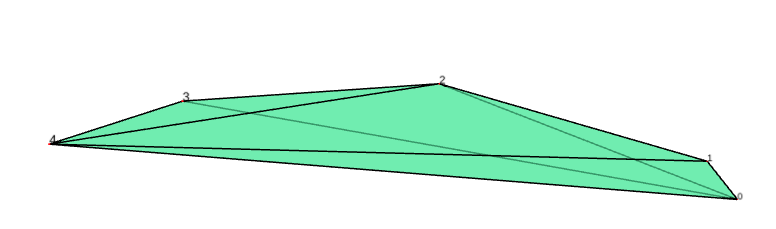
\includegraphics[width=.30\textwidth, height=0.4\textheight]{images/cyclic}
  \end{center}
\end{frame}
%%%%%%%%%%%%%%%%%%%%%%%%%%%%%%%%%%%%%%%%%%%%%%%%%%%%%%%%%%%%%%%%%%%%%%%%%%%%%%%
%%%%%%%%%%%%%%%%%%%%%%%%%%%%%%%%%%%%%%%%%%%%%%%%%%%%%%%%%%%%%%%%%%%%%%%%%%%%%%%
%%%%%%%%%%%%%%%%%%%%%%%%%%%%%%%%%%%%%%%%%%%%%%%%%%%%%%%%%%%%%%%%%%%%%%%%%%%%%%%

\begin{frame}[fragile]{A Partitioning Lemma}
  \begin{lemma}
    Let $P = \text{conv}V$, and let $P' = P \cap H^+$, where $H$ is a hyperplane. \\
    Let $V_0, V_+, V_-$ be the partition of a point set $V$, defined by
    \begin{center}
      $V_0 = V \cap H, V_+ = V \cap H^+ \setminus H, V_- = V \cap H^- \setminus H$
    \end{center}
    where $H$ is a hyperplane. Then we have
    \begin{center}
      $P' \cap H^+ =
      \text{conv}(V_0 \cup V_+ \cup \set{[v, w] \cap H \mid v \in V_+ , w \in V_-})$
      \end{center}
  \end{lemma}
    \begin{center}
    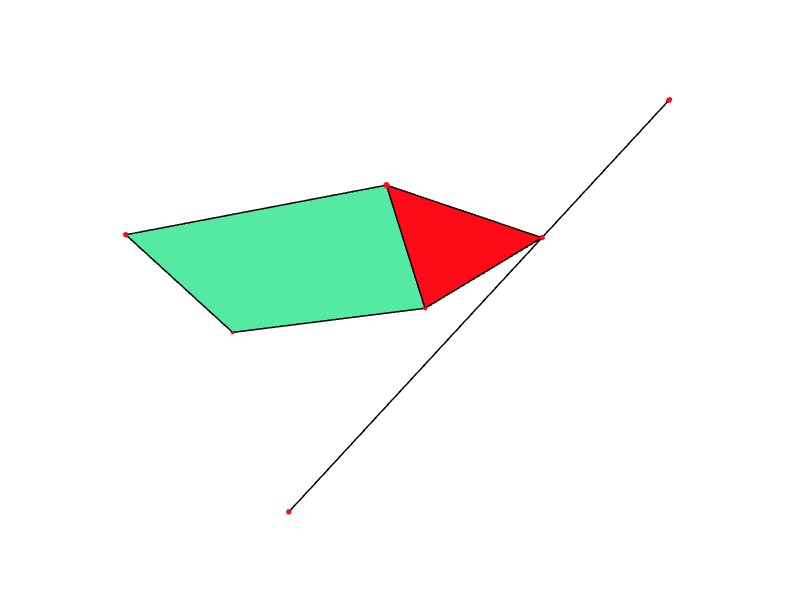
\includegraphics[width=.50\textwidth, height=0.4\textheight]{images/lemma}
  \end{center}
\end{frame}
%%%%%%%%%%%%%%%%%%%%%%%%%%%%%%%%%%%%%%%%%%%%%%%%%%%%%%%%%%%%%%%%%%%%%%%%%%%%%%%
%%%%%%%%%%%%%%%%%%%%%%%%%%%%%%%%%%%%%%%%%%%%%%%%%%%%%%%%%%%%%%%%%%%%%%%%%%%%%%%
%%%%%%%%%%%%%%%%%%%%%%%%%%%%%%%%%%%%%%%%%%%%%%%%%%%%%%%%%%%%%%%%%%%%%%%%%%%%%%%

\begin{frame}[fragile]{A Basic Algorithm }
  \begin{algorithm}[H]
    \textbf{Input:} A set of affine half-spaces $\mathcal{H} = \set{H_1^+, \dots, H_m^+}$
    in $\R^n$ such that $P = \cap_{i=1}^m H_i^+$ is bounded and full dimensional
    and $P_{n+1} = \cap_{i=1}^{n+1}H_i^+$ is an $n$-simplex\\
    \textbf{Output:} Point set $V$ such that $\text{conv}V = P$
    \begin{algorithmic}[1]
      \STATE $V_{n+1} \leftarrow$ set of vertices of $P_{n+1}$
      \FOR{$k=n+2$ to $m$}
      \STATE Construct $V_k$ such that $\text{conv}V_k = P_k = P_{k-1} \cap H_k^+$ as in the lemma
      \ENDFOR
    \end{algorithmic}
  \end{algorithm}
\end{frame}
%%%%%%%%%%%%%%%%%%%%%%%%%%%%%%%%%%%%%%%%%%%%%%%%%%%%%%%%%%%%%%%%%%%%%%%%%%%%%%%
%%%%%%%%%%%%%%%%%%%%%%%%%%%%%%%%%%%%%%%%%%%%%%%%%%%%%%%%%%%%%%%%%%%%%%%%%%%%%%%
%%%%%%%%%%%%%%%%%%%%%%%%%%%%%%%%%%%%%%%%%%%%%%%%%%%%%%%%%%%%%%%%%%%%%%%%%%%%%%%

\begin{frame}[fragile]{}
  \begin{itemize}
  \item The basic algorithm is an improvement on the trivial one.
  \item The basic algorithm uses points that aren't vertices.
  \item At each iteration we may have that the points increase quadratically.
  \item Improvements can be made by noticing that vertices of $P_k$ which are not vertices of $P_{k-1}$ are generated by edges of $P_{k-1}$ that intersect the hyperplane $H_k$
  \end{itemize}
\end{frame}

%%%%%%%%%%%%%%%%%%%%%%%%%%%%%%%%%%%%%%%%%%%%%%%%%%%%%%%%%%%%%%%%%%%%%%%%%%%%%%%
%%%%%%%%%%%%%%%%%%%%%%%%%%%%%%%%%%%%%%%%%%%%%%%%%%%%%%%%%%%%%%%%%%%%%%%%%%%%%%%
%%%%%%%%%%%%%%%%%%%%%%%%%%%%%%%%%%%%%%%%%%%%%%%%%%%%%%%%%%%%%%%%%%%%%%%%%%%%%%%

\begin{frame}[fragile]{Edge Detecting Lemma }
  \begin{defn}
    Let $W \subset V$ be a point set and define $\mathcal{H}(W) = \set{H \mid H = \partial H^+ \text{ for } H \in \mathcal{H^+} \text{ and } W \subset H}$. For simplicity we denote $H(\set{v, w})$ as $H(v, w)$
  \end{defn}
  \begin{lemma}
    Let $(V, \mathcal{H})$ be a double description of an $n$-polytope $P$. Given two distinct points $v, w \in V$ the set aff$\set{v, w} \cap P$ is an edge of $P$ if and only if
    \begin{center}
      $\cap \mathcal{H}(v, w) = \text{aff}\set{v, w}$.
    \end{center}

    
    When $v, w$ are vertices then
    \begin{center}
      conv$\set{v, w} = P \cap (\cap \mathcal{H}(v, w))$
    \end{center}
  \end{lemma}
\end{frame}

%%%%%%%%%%%%%%%%%%%%%%%%%%%%%%%%%%%%%%%%%%%%%%%%%%%%%%%%%%%%%%%%%%%%%%%%%%%%%%%
%%%%%%%%%%%%%%%%%%%%%%%%%%%%%%%%%%%%%%%%%%%%%%%%%%%%%%%%%%%%%%%%%%%%%%%%%%%%%%%
%%%%%%%%%%%%%%%%%%%%%%%%%%%%%%%%%%%%%%%%%%%%%%%%%%%%%%%%%%%%%%%%%%%%%%%%%%%%%%%

\begin{frame}[fragile]{Finding a Data Structure}
  \begin{itemize}
  \item We would like to find the right data structure that allows us to take
    advantage of lemma
  \item We would like to change finding dimension to finding the rank of a matrix
  \item Using homogeneous coordinates allows us to change from affine space to a linear space
  \item We will need to extend convex hull problem to pointed polyhedron
  \end{itemize}
\end{frame}

%%%%%%%%%%%%%%%%%%%%%%%%%%%%%%%%%%%%%%%%%%%%%%%%%%%%%%%%%%%%%%%%%%%%%%%%%%%%%%%
%%%%%%%%%%%%%%%%%%%%%%%%%%%%%%%%%%%%%%%%%%%%%%%%%%%%%%%%%%%%%%%%%%%%%%%%%%%%%%%
%%%%%%%%%%%%%%%%%%%%%%%%%%%%%%%%%%%%%%%%%%%%%%%%%%%%%%%%%%%%%%%%%%%%%%%%%%%%%%%


\begin{frame}[fragile]{Homogenizing}
  We now let $P$ be an $n$-dimensional point polyhedron and homogenize by considering
  \begin{center}
    $Q  = \set{(\lambda, \lambda x) \mid x \in P}$
  \end{center}
  We know $P = \text{conv}V + \text{pos}R$, and so $Q$ can be described as
  \begin{center}
    $Q = \text{pos}(\set{(1, v) \mid v \in V} \cup \set{(0, r) \mid r \in R})$
  \end{center}
  \begin{defn}
    \begin{itemize}
      \item We define $W$ to be the set of vectors that generate $Q$, and we store $W$
    as an $(n+1) \times m$ matrix, where the columns are the vectors $w^{(i)}$.\\
    \item We define the $k \times(n+1)$ matrix $\mathcal{H}$ to be the matrix whose
      rows are the linear half-spaces $h^{(i)}$.
    \end{itemize}
  \end{defn}
\end{frame}

%%%%%%%%%%%%%%%%%%%%%%%%%%%%%%%%%%%%%%%%%%%%%%%%%%%%%%%%%%%%%%%%%%%%%%%%%%%%%%%
%%%%%%%%%%%%%%%%%%%%%%%%%%%%%%%%%%%%%%%%%%%%%%%%%%%%%%%%%%%%%%%%%%%%%%%%%%%%%%%
%%%%%%%%%%%%%%%%%%%%%%%%%%%%%%%%%%%%%%%%%%%%%%%%%%%%%%%%%%%%%%%%%%%%%%%%%%%%%%%

\begin{frame}[fragile]{Incidence Matrix}
  \begin{defn}
    Let $(W, \mathcal{H})$ be a double description of a pointed cone $Q \subset \R^{n+1}$
    with $W \in \R^{(n+1) \times m}$ and $\mathcal{H} \in \R^{k \times (n+1)}$. The \emph{incidence matrix} $I(W, \mathcal{H})$ is defined as
    
    \begin{equation}
      I_{ij}=
      \begin{cases}
        1 & \text{if } w^{(j)} \in H_i = \partial H_i^+, i.e., h^{(j)} (w^{(i)}) = 0\\
        0 &  \text{otherwise}
      \end{cases}
    \end{equation}
  \end{defn}
  \begin{remark}
    We use $I(W, \mathcal{H})$ to quickly determine the set $\mathcal{H}(w^{(s)}, w^{(t)})$. Then we can calculate the dimension of the intersection of the half-spaces as $n+1$ minus the rank of the submatrix $\mathcal{H}(w^{(s)}, w^{(t)})$
  \end{remark}
\end{frame}

%%%%%%%%%%%%%%%%%%%%%%%%%%%%%%%%%%%%%%%%%%%%%%%%%%%%%%%%%%%%%%%%%%%%%%%%%%%%%%%
%%%%%%%%%%%%%%%%%%%%%%%%%%%%%%%%%%%%%%%%%%%%%%%%%%%%%%%%%%%%%%%%%%%%%%%%%%%%%%%
%%%%%%%%%%%%%%%%%%%%%%%%%%%%%%%%%%%%%%%%%%%%%%%%%%%%%%%%%%%%%%%%%%%%%%%%%%%%%%%
\begin{frame}[fragile]{Double Description Algorithm}
  \begin{center}
    \includegraphics[width=.90\textwidth, height=0.85\textheight]{images/algorithm}
  \end{center}
\end{frame}


%%%%%%%%%%%%%%%%%%%%%%%%%%%%%%%%%%%%%%%%%%%%%%%%%%%%%%%%%%%%%%%%%%%%%%%%%%%%%%%
\section{Current State of Convex Hull Computations}
%%%%%%%%%%%%%%%%%%%%%%%%%%%%%%%%%%%%%%%%%%%%%%%%%%%%%%%%%%%%%%%%%%%%%%%%%%%%%%%

\begin{frame}[fragile]{Bad News}
  \begin{itemize}
  \item It's hard.
  \item No globally optimal algorithm is known.
  \item Difficult to say which algorithm works best on what input.
  \item It is not known if there exists a polynomial total time algorithm (polynomial in input and output)
  \item No incremental algorithm can run in polynomial total time
  \end{itemize}
\end{frame}



%%%%%%%%%%%%%%%%%%%%%%%%%%%%%%%%%%%%%%%%%%%%%%%%%%%%%%%%%%%%%%%%%%%%%%%%%%%%%%%
%%%%%%%%%%%%%%%%%%%%%%%%%%%%%%%%%%%%%%%%%%%%%%%%%%%%%%%%%%%%%%%%%%%%%%%%%%%%%%%
%%%%%%%%%%%%%%%%%%%%%%%%%%%%%%%%%%%%%%%%%%%%%%%%%%%%%%%%%%%%%%%%%%%%%%%%%%%%%%%

\begin{frame}[fragile]{Good News}
  State of the art algorithms are available in \texttt{polymake}, hence OSCAR.
  Here is a short list on noteable algorithms 
  \begin{itemize}
  \item Beneath and beyond, ``beneath\_beyond'' (incremental).
  \item Double description, ``cdd'', ``ppl''(incremental).
  \item Pyramid Decomposition, ``libnormaliz'' (incremental).
  \item Reverse Search ``lrs''.
      
  \end{itemize}
\end{frame}

%%%%%%%%%%%%%%%%%%%%%%%%%%%%%%%%%%%%%%%%%%%%%%%%%%%%%%%%%%%%%%%%%%%%%%%%%%%%%%%
%%%%%%%%%%%%%%%%%%%%%%%%%%%%%%%%%%%%%%%%%%%%%%%%%%%%%%%%%%%%%%%%%%%%%%%%%%%%%%%
%%%%%%%%%%%%%%%%%%%%%%%%%%%%%%%%%%%%%%%%%%%%%%%%%%%%%%%%%%%%%%%%%%%%%%%%%%%%%%%

\begin{frame}[fragile]{Rules of Thumb}
  \begin{itemize}
  \item If you don't know anything try double description.
  \item If you expect the output to be extremely large and if partial information is
    useful.
  \item Use double description when looking for facets of $0 / 1$ polytopes.
  \item Beneath and beyond often behaves well on random input.
  \end{itemize}

\end{frame}

%%%%%%%%%%%%%%%%%%%%%%%%%%%%%%%%%%%%%%%%%%%%%%%%%%%%%%%%%%%%%%%%%%%%%%%%%%%%%%%
%%%%%%%%%%%%%%%%%%%%%%%%%%%%%%%%%%%%%%%%%%%%%%%%%%%%%%%%%%%%%%%%%%%%%%%%%%%%%%%
%%%%%%%%%%%%%%%%%%%%%%%%%%%%%%%%%%%%%%%%%%%%%%%%%%%%%%%%%%%%%%%%%%%%%%%%%%%%%%%

\begin{frame}[fragile]
  \begin{center}
    Thank you!
  \end{center}
\end{frame}

\begin{frame}
  \frametitle{References}
  \footnotesize{
    \begin{thebibliography}{99} % Beamer does not support BibTeX so references must be inserted manually as below
    \bibitem[Joswig, Thorsten, 2013]{p1} Michael Joswig, Thorsten Theobald, (2013)
      \newblock Polyhedral and algebraic methods in computational geometry
      \newblock London: Springer

    \bibitem[chulls 2017]{p1} Assarf, Benjamin and Gawrilow, Ewgenij and Herr, Katrin and Joswig, Michael and Lorenz, Benjamin and Paffenholz, Andreas and Rehn, Thomas, (2017)
      \newblock Computing convex hulls and counting integer points with \texttt{polymake}
      \newblock Mathematical Programming Computation 9(1), 1--38 



  \end{thebibliography}
  }
\end{frame}

%%%%%%%%%%%%%%%%%%%%%%%%%%%%%%%%%%%%%%%%%%%%%%%%%%%%%%%%%%%%%%%%%%%%%%%%%%%%%%%
%%%%%%%%%%%%%%%%%%%%%%%%%%%%%%%%%%%%%%%%%%%%%%%%%%%%%%%%%%%%%%%%%%%%%%%%%%%%%%%
%%%%%%%%%%%%%%%%%%%%%%%%%%%%%%%%%%%%%%%%%%%%%%%%%%%%%%%%%%%%%%%%%%%%%%%%%%%%%%%

\end{document}
